% 图 8.20 Fe/Cr/Fe 三明治：(a) H > H_s 两 Fe 层磁矩平行 (b) H = 0、t_Cr 适当时反平行
\documentclass[tikz,border=5pt]{standalone}
\usetikzlibrary{arrows.meta}
\usepackage{amsmath}
\usepackage{bm}
\usepackage{fontspec}
\setmainfont{Times New Roman}
\begin{document}
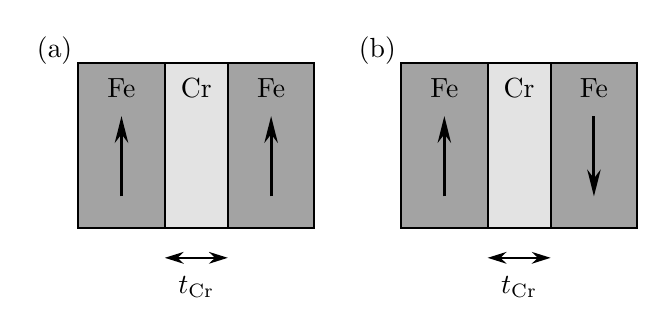
\begin{tikzpicture}[line width=0.8pt,>=Stealth]
% ---------- (a) parallel moments ----------
\begin{scope}[shift={(0,0)}]
  \fill[gray!72] (0,0) rectangle (1.1,2.1);
  \fill[gray!22] (1.1,0) rectangle (1.9,2.1);
  \fill[gray!72] (1.9,0) rectangle (3.0,2.1);
  \draw[line width=0.7] (0,0) rectangle (3.0,2.1);
  \draw[line width=0.7] (1.1,0) -- (1.1,2.1);
  \draw[line width=0.7] (1.9,0) -- (1.9,2.1);
  \node at (0.55,1.78) {Fe};
  \node at (1.5,1.78) {Cr};
  \node at (2.45,1.78) {Fe};
  \draw[->,line width=1.1,-{Stealth[length=3.4mm,width=1.7mm]}]
    (0.55,0.4) -- (0.55,1.42);
  \draw[->,line width=1.1,-{Stealth[length=3.4mm,width=1.7mm]}]
    (2.45,0.4) -- (2.45,1.42);
  \draw[{Stealth[length=2.4mm,width=1.5mm]}-{Stealth[length=2.4mm,width=1.5mm]},line width=0.7]
    (1.1,-0.38) -- (1.9,-0.38);
  \node at (1.5,-0.75) {$t_{\mathrm{Cr}}$};
  \node at (-0.3,2.25) {(a)};
\end{scope}
% ---------- (b) antiparallel moments ----------
\begin{scope}[shift={(4.1,0)}]
  \fill[gray!72] (0,0) rectangle (1.1,2.1);
  \fill[gray!22] (1.1,0) rectangle (1.9,2.1);
  \fill[gray!72] (1.9,0) rectangle (3.0,2.1);
  \draw[line width=0.7] (0,0) rectangle (3.0,2.1);
  \draw[line width=0.7] (1.1,0) -- (1.1,2.1);
  \draw[line width=0.7] (1.9,0) -- (1.9,2.1);
  \node at (0.55,1.78) {Fe};
  \node at (1.5,1.78) {Cr};
  \node at (2.45,1.78) {Fe};
  \draw[->,line width=1.1,-{Stealth[length=3.4mm,width=1.7mm]}]
    (0.55,0.4) -- (0.55,1.42);
  \draw[->,line width=1.1,-{Stealth[length=3.4mm,width=1.7mm]}]
    (2.45,1.42) -- (2.45,0.4);
  \draw[{Stealth[length=2.4mm,width=1.5mm]}-{Stealth[length=2.4mm,width=1.5mm]},line width=0.7]
    (1.1,-0.38) -- (1.9,-0.38);
  \node at (1.5,-0.75) {$t_{\mathrm{Cr}}$};
  \node at (-0.3,2.25) {(b)};
\end{scope}
\end{tikzpicture}
\end{document}
